
\section{Decision trees. Random fores. Bagging, boosting.}



	
	\subsection{Decision Trees}
	A single Decision Tree splits data hierarchically based on feature thresholds until it reaches a terminal leaf node.
	
	\begin{center}
		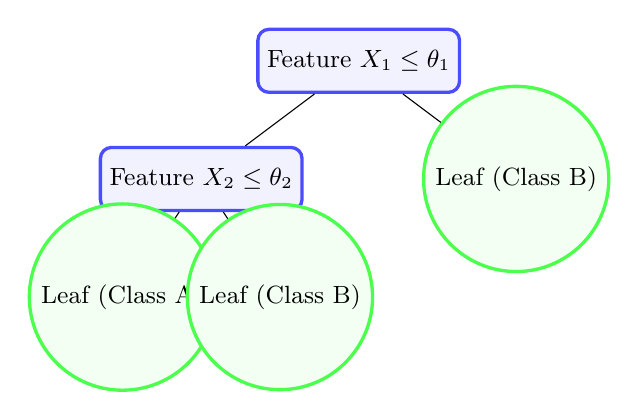
\begin{tikzpicture}[
		level distance=1.5cm,
		level 1/.style={sibling distance=4cm},
		level 2/.style={sibling distance=2cm},
		internal/.style={rectangle, draw=blue!70, fill=blue!5, very thick, rounded corners, minimum size=0.8cm, font=\small},
		leaf/.style={circle, draw=green!70, fill=green!5, very thick, minimum size=0.8cm, font=\small}
		]
		% Root Node
		\node[internal] {Feature $X_1 \le \theta_1$}
		child { node[internal] {Feature $X_2 \le \theta_2$} 
			child { node[leaf] {Leaf (Class A)} }
			child { node[leaf] {Leaf (Class B)} }
		}
		child { node[leaf] {Leaf (Class B)} };
		\end{tikzpicture}
	\end{center}	

	Nodes are split by maximizing Information Gain or minimizing Impurity. 
	
	\begin{itemize}
		\item \textbf{Gini Impurity} (for a node $D$ with $C$ classes):
		\begin{equation}
		\text{Gini}(D) = 1 - \sum_{i=1}^{C} p_i^2
		\end{equation}
		where $p_i$ is the probability of an item belonging to class $i$.
		
		\item \textbf{Entropy}:
		\begin{equation}
		H(D) = - \sum_{i=1}^{C} p_i \log_2 p_i
		\end{equation}
		
		\item \textbf{Information Gain} from a split on feature $A$:
		\begin{equation}
		\text{Gain}(D, A) = H(D) - \sum_{v \in \text{Values}(A)} \frac{|D_v|}{|D|} H(D_v)
		\end{equation}
	\end{itemize}
	
	\newpage
	
	\subsection{Random Forest Architecture}
	A Random Forest grows an ensemble of $B$ independent decision trees via bagging (bootstrap aggregating) and feature randomness, then combines their outputs.
	
	\begin{center}
		\begin{tikzpicture}[
		box/.style={draw=black!70, rectangle, minimum width=2.2cm, minimum height=1cm, align=center, rounded corners, font=\small},
		arrow/.style={-{Stealth[scale=1.2]}, thick, draw=black!80}
		]
		% Input Layer
		\node[box, fill=purple!5, draw=purple!70, ultra thick] (input) {Input Dataset \\ $\mathbf{x} = [x_1, x_2, \dots, x_d]$};
		
		% Ensemble Layer
		\node[box, fill=blue!5, below=1.2cm of input, xshift=-3.5cm] (tree1) {\textbf{Decision Tree 1} \\ $\hat{y}_1 = h_1(\mathbf{x})$};
		\node[box, fill=blue!5, below=1.2cm of input, xshift=-0.5cm] (tree2) {\textbf{Decision Tree 2} \\ $\hat{y}_2 = h_2(\mathbf{x})$};
		\node[draw=none, right=0.4cm of tree2, yshift=-0.2cm] (dots) {\textbf{\dots}};
		\node[box, fill=blue!5, below=1.2cm of input, xshift=3.5cm] (treeB) {\textbf{Decision Tree $B$} \\ $\hat{y}_B = h_B(\mathbf{x})$};
		
		% Aggregation Layer
		\node[box, fill=orange!5, draw=orange!70, ultra thick, below=3.2cm of input] (agg) {\textbf{Aggregation Node} \\ (Majority Vote / Averaging)};
		
		% Output Layer
		\node[box, fill=green!5, draw=green!70, ultra thick, below=1.0cm of agg] (output) {Final Prediction \\ $\hat{y}$};
		
		% Connections
		\draw[arrow] (input.south) -- (tree1.north);
		\draw[arrow] (input.south) -- (tree2.north);
		\draw[arrow] (input.south) -- (treeB.north);
		
		\draw[arrow] (tree1.south) -- (agg.west);
		\draw[arrow] (tree2.south) -- (agg.north);
		\draw[arrow] (treeB.south) -- (agg.east);
		
		\draw[arrow] (agg) -- (output);
		\end{tikzpicture}
	\end{center}
	
	Let $h_b(\mathbf{x})$ be the prediction of the $b$-th operational decision tree.
	
	\begin{itemize}
		\item \textbf{Classification (Majority Voting)}:
		\begin{equation}
		\hat{y} = \text{mode} \Big\{ h_1(\mathbf{x}), h_2(\mathbf{x}), \dots, h_B(\mathbf{x}) \Big\}
		\end{equation}
		
		\item \textbf{Regression (Ensemble Averaging)}:
		\begin{equation}
		\hat{y} = \frac{1}{B} \sum_{b=1}^{B} h_b(\mathbf{x})
		\end{equation}
	\end{itemize}
	

	
\newpage